\documentclass{article}
\makeatletter
\def\input@path{{ISBI_template-master/}{Assignment 3 - Group/report/ISBI_template-master/}}
\makeatother
\usepackage{spconf}
\usepackage{amsmath,amssymb,graphicx}
\usepackage{multirow}
\usepackage{booktabs,array,longtable}
\usepackage[hidelinks]{hyperref}
\graphicspath{{figures/}{Assignment 3 - Group/report/figures/}}
\setlength{\parindent}{0pt}
\pagestyle{plain}

\title{Video-Conditioned 3D Object Reconstruction}
\name{\shortstack{Group 15: Hans Peter Lyngsøe, Harald Franck, \\ Mathias Elmegaard Nielsen and Julian Barragan}}
\address{Assignment 3: Mini Research Report \\
\small\textit{Baseline paper: SAM 3D\cite{sam3d}, Course-curated paper: V-JEPA\cite{vjepa21}} \\
\small\url{https://github.com/HP2706/ATDL-Group-Work}}


\begin{document}
\maketitle

\begin{abstract}
Recent breakthroughs in vision foundation models, notably SAM3 and SAM 3D, have substantially advanced single-image 3D object reconstruction. However, occluded parts of objects must be inferred from learned priors rather than observed evidence. Recent approaches have proposed training-free multi-view extensions to address this limitation by fusing predictions conditioned on different images. However these techniques remain limited in two ways. First they require repeated forward passes through the main backbone, leading to poor computational efficiency. Secondly for these methods to work, one needs a separate heuristic or models for selecting informative frames, hindering usability. We propose a lightweight adapter that conditions SAM 3D directly on video representations extracted by the pretrained V-JEPA 2.1 encoder. This architecture avoids per-view generator evaluations at each sampling step and remove the dependence on frame selection in the input pipeline. We investigate whether this approach improves coarse object reconstruction, particularly for surfaces revealed beyond the reference view.

\end{abstract}

\section{Introduction}
Foundation models for single-image 3D reconstruction, most notably SAM 3D~\cite{sam3d}, recover the complete geometry of a masked object from one photograph. Surfaces that are not visible in that image, however, must be inferred from learned shape priors, and front--back ambiguity remains a central source of error~\cite{front2back}. A short video of the object often observes exactly these surfaces, but SAM 3D can only be conditioned on a single image. In this paper, we thus propose a method for extending SAM 3D to video inputs by encoding a clip with the frozen self-supervised video encoder V-JEPA~2.1~\cite{vjepa21} and injecting its features into the conditioning tokens of SAM 3D's geometry model through a lightweight adapter. To address, whether a pretrained foundation model can accept a new input modality through a small adapter without losing its learned prior, and whether any resulting gain reflects the video itself or merely adaptation to the training domain, we formulate the following research questions and hypotheses:

\textbf{Research question.} Can a lightweight adapter on frozen V-JEPA~2.1 features inject video evidence into SAM 3D and improve coarse geometry over (a) frozen SAM 3D, (b) an image-only fine-tuning control with the same training budget, and (c) training-free multi-view fusion, and how should the video features enter the conditioning sequence? We test three hypotheses:
\begin{itemize}
  \item[\textbf{H1}] In distribution, video conditioning improves coarse geometry over frozen SAM 3D, even with SAM 3D frozen, and over an image-only LoRA control, so that the gain is attributable to video evidence rather than domain adaptation.
  \item[\textbf{H2}] The improvement transfers to scanned real-world objects (GSO), where the learned single-pass fusion matches or exceeds training-free multi-view fusion.
  \item[\textbf{H3}] Strategies that preserve SAM 3D's native conditioning tokens outperform strategies that replace them, and identity-initialized gated fusion is the most robust.
\end{itemize}

\textbf{Contributions.} (i) Three strategies for conditioning SAM 3D on V-JEPA~2.1 video features (gated fusion, attention pooling, and appended tokens), each requiring a single backbone evaluation per flow step; (ii) a synthetic dataset of 10,000 rendered multi-object clips with exact masks and complete 3D geometry; (iii) a controlled comparison against frozen SAM 3D, two training-free multi-view methods, and a matched image-only fine-tuning control on held-out synthetic data and GSO, with paired bootstrap confidence intervals; (iv) the finding that video conditioning improves reconstruction in distribution but does not transfer to GSO, and that preserving the native conditioning tokens is essential.

\section{Related Work}

\subsection{SAM3D}

\subsubsection{Data Generation}

A central challenge in image-conditioned 3D reconstruction is obtaining images paired with complete object geometry. SAM 3D addresses this during pretraining with Iso-3DO, a dataset built from 2.7 million meshes from Objaverse-XL and licensed sources~\cite{sam3d}. Each mesh is rendered from 24 viewpoints as an isolated, centered object, yielding (image,shape,texture) triplets. Each image and the  underlying mesh is then paired. In order to encourage robustness to partial occlusion, they 
introduce samples during mid-training where the objects of interest are partly occluded.

\subsubsection{Architecture}

SAM 3D reconstructs geometry, appearance, and layout from an image $I$ and target-object mask $M$ using two conditional flow models~\cite{sam3d}. A pretrained DINOv2 encoder separately encodes four inputs: the full image, the object crop, the full-image mask, and the cropped mask. Each input group $g$ produces a token sequence $E_g\in\mathbb{R}^{N_g\times d_{\mathrm{DINO}}}$, where $N_g$ is its number of tokens and $d_{\mathrm{DINO}}$ is the encoder feature width. An optional scene point map provides an additional token sequence. Each group is projected to a common width and augmented with a learned embedding identifying its source:
\begin{equation}
    C_G=\operatorname{Concat}_{\mathrm{tokens}}\!\left(
    \{\Pi_g(E_g)+e_g\}_{g\in\mathcal{G}}
    \right)\in\mathbb{R}^{N_c\times d_c},
\end{equation}
where $\mathcal{G}$ indexes the four image and mask groups and the optional point-map group, $\Pi_g$ is a learned per-token projection, and $e_g$ is the group embedding. Concatenation preserves the individual tokens, giving a conditioning sequence of $N_c$ tokens with width $d_c$. The geometry model accesses this sequence through cross-attention: its current shape and layout tokens form the queries, while $C_G$ supplies the keys and values. This conditioning sequence is the interface through which our adapter introduces video evidence.

The geometry model iteratively transforms noise into a coarse shape latent and object rotation, translation, and scale. The shape latent is decoded into a $64^3$ occupancy grid. A second conditional flow model generates features on the occupied voxels, which are decoded into a textured mesh or Gaussian splats. Our experiments train video conditioning for the geometry model while keeping the refinement model frozen.

\subsection{Video Representation Learning}

V-JEPA 2.1 learns by predicting video features rather than pixels~\cite{vjepa21}. Given a clip $x$, the context encoder $f:x_{\mathcal C}\mapsto H_{\mathcal C}$ encodes its visible tokens. The predictor $p:(H_{\mathcal C},\Delta_{\mathcal M})\mapsto\widehat H$ uses these features and positional mask tokens $\Delta_{\mathcal M}$ to predict features at all positions. A moving-average teacher encodes the complete clip to provide stop-gradient targets $h_i$. With prediction error $e_i=\|\widehat h_i-h_i\|_1$, training minimizes
\begin{equation}
    \mathcal L_{\mathrm{dense}}=
    \frac{1}{|\mathcal M|}\sum_{i\in\mathcal M}e_i
    +\frac{1}{|\mathcal C|}\sum_{i\in\mathcal C}\lambda_i e_i,
\end{equation}
where $\mathcal M$ and $\mathcal C$ index masked and visible tokens. Unlike earlier V-JEPA models, version 2.1 also supervises visible tokens, weighting those near masked regions more heavily through $\lambda_i$. Supervision at multiple encoder depths further improves dense spatial features while retaining video understanding.

\subsection{Multi-View 3D Reconstruction}



MV-SAM3D~\cite{mvsam3d} extends frozen SAM 3D to multiple input views without additional training. At each flow step, it evaluates the velocity field separately for each view's conditioning $C_i$, while keeping the current latent state $z_\tau$ fixed. The resulting predictions are combined at each latent token $q$ by a weighted combination:
\begin{equation}
\begin{aligned}
    \overline v_\theta(z_\tau,\tau)_q
        &=\sum_{i=1}^{N}w_i(q)\,v_\theta(z_\tau,\tau,C_i)_q,\\
    \sum_{i=1}^{N}w_i(q)&=1.
\end{aligned}
\end{equation}

for computing non-uniform weight, they use a technique called 'attention-entropy weighting' where greater weight is assigned to views with more concentrated cross-attention .
\begin{equation}
    w_i(q)=\frac{\exp[-\alpha H_i(q)]}
    {\sum_{j=1}^{N}\exp[-\alpha H_j(q)]},
\end{equation}
where $H_i(q)$ is the normalized entropy of token $q$'s attention over view $i$'s image patches, and $\alpha$ controls the weighting sharpness.

Stream3D~\cite{stream3d} extends frozen SAM 3D to streaming inputs without additional training. For each chunk, it probes SAM 3D's structure-stage flow model from fixed noise. Cross-attention between 3D grid tokens and image patches yields evidence scores $e_i(q)$, rewarding strong, concentrated attention. Each token's memory stores its $D$ highest scores and corresponding frame indices, updated for chunk $\mathcal C_k$ as
\begin{equation}
    \mathcal M_k(q)=\operatorname{TopD}_{e}\!\left(
    \mathcal M_{k-1}(q)\cup\{(e_i(q),i):i\in\mathcal C_k\}
    \right).
\end{equation}
The $K$ frames appearing most often in memory form $\mathcal V_k$. Reconstruction starts from fresh noise; SAM 3D predicts per-view velocities at the shared latent $z_\tau$ and fuses them using normalized evidence:
\begin{equation}
\begin{aligned}
    \overline v_\theta(z_\tau,\tau)_q
        &=\sum_{i\in\mathcal V_k}w_i(q)\,v_\theta(z_\tau,\tau,C_i)_q,\\
    w_i(q)&=\frac{e_i(q)}{\sum_{j\in\mathcal V_k}e_j(q)}.
\end{aligned}
\end{equation}
Thus, historical frame references and scores persist across chunks, while SAM 3D generates a new reconstruction from the selected observations.

Both methods therefore incorporate information from multiple observations into a shared latent $z_\tau$ during sampling. Each forward pass predicts a velocity; the solver updates the latent, for example with an Euler step:
\begin{equation}
    z_{\tau+\Delta\tau}=z_\tau+\Delta\tau\,\overline v_\theta(z_\tau,\tau).
\end{equation}
Our approach instead learns to combine video evidence in the conditioning sequence before these sampling steps.


\section{Method}
\begin{figure*}[t]
  \centering
  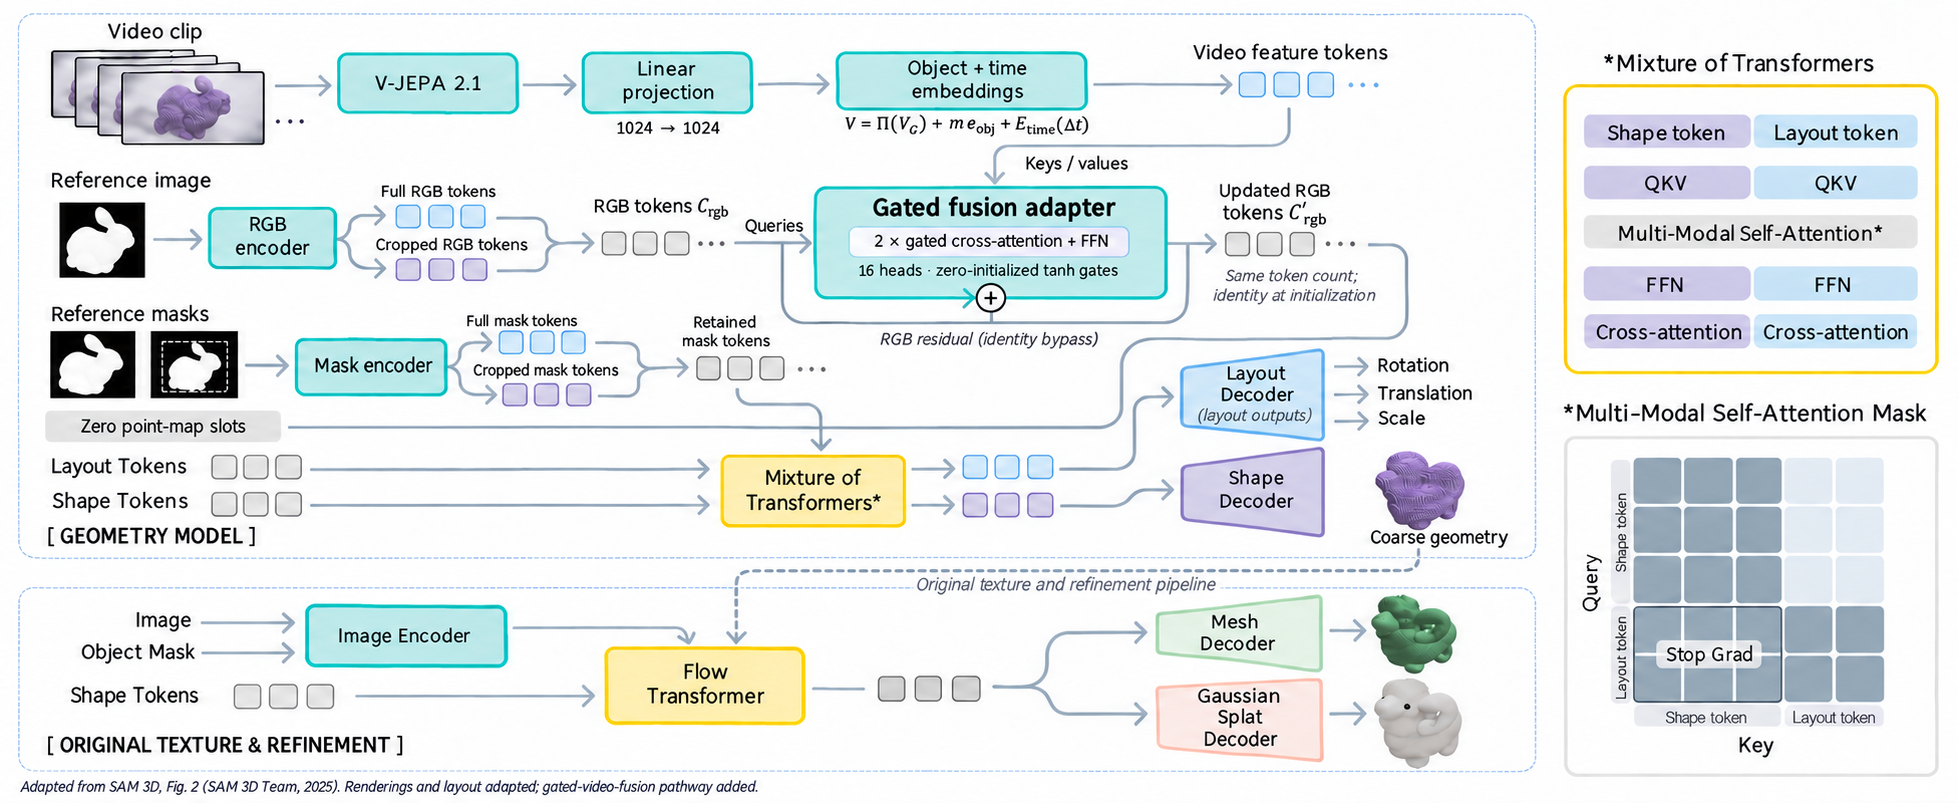
\includegraphics[width=\textwidth]{fusion_adapter_source_style_v2.png}
  \caption{Gated fusion of video features into SAM 3D conditioning. V-JEPA 2.1 video features are projected and augmented with object-coverage and temporal embeddings. Two gated cross-attention blocks update the native RGB conditioning tokens, using RGB tokens as queries and video features as keys and values. Zero-initialized gates preserve the original conditioning at initialization. Mask tokens and zero point-map slots are retained. Adapted from Figure 2 of SAM 3D~\cite{sam3d}.}
  \label{fig:fusion-adapter}
\end{figure*}

\subsection{Data Generation}


\subsection{Architecture}

In order to condition SAM 3D on video, we must incorporate this information into the conditioning tokens provided to the model backbone. We use VJEPA2.1 \cite{vjepa21} to obtain video-embeddings.

Let $V_G=f_{\theta_V}(I_{1:K})\in\mathbb{R}^{N_v\times d_v}$ denote the video embeddings for a clip of $K$ frames with $N_v$ as the number of spatiotemporal tokens and $d_v$ as the encoder feature width. For V-JEPA 2.1 ViT-L/16 using final-layer features, $d_v=1024$ and $N_v=T_v(H_v/16)(W_v/16)$, where $T_v=K/2$ for even $K>1$ and $T_v=1$ for a single frame. Framewise DINOv2 variants instead use $14\times14$ spatial patches.

We compare three strategies for incorporating video information: updating the native RGB tokens through gated fusion, replacing them with pooled video tokens, and appending video and mask tokens. We hypothesize that extending the conditioning sequence may be more disruptive to the pretrained backbone and require backbone weight updates.

Recall that
\begin{equation}
    C_G=\operatorname{Concat}_{\mathrm{tokens}}\!
    \left(C_{\mathrm{rgb}},C_{\mathrm{mask}},[C_{\mathrm{pointmap}}]\right)
    \in\mathbb{R}^{N_c\times1024},
\end{equation}
where $[\cdot]$ indicates an optional input and
\begin{equation}
    C_{\mathrm{rgb}}=\operatorname{Concat}_{\mathrm{tokens}}\!
    \left(C_{\mathrm{full,rgb}},C_{\mathrm{crop,rgb}}\right)
    \in\mathbb{R}^{N_{\mathrm{rgb}}\times1024}.
\end{equation}

Gated fusion and video pooling modify only $C_{\mathrm{rgb}}$, retaining the mask and optional point-map streams:
\begin{equation}
    a_{\theta_A}:(C_{\mathrm{rgb}},V_G)\longmapsto C_{\mathrm{rgb}}'.
\end{equation}
Gated fusion preserves the $N_{\mathrm{rgb}}$ RGB tokens, while video pooling replaces them with $64$ pooled tokens. The appended-token strategy instead retains all native streams and adds video and mask summaries. Each strategy produces conditioning $C_G'$, which is reused at every flow step in $v_{\theta_G}(x_\tau,\tau,C_G')$. The concatenation above groups tokens by modality for notation; the native fuser concatenates the individual streams in one operation.

\subsection{Fusion Adapter}

Each video token is projected to the conditioning width and augmented with object coverage $m_i$ and relative frame offset $\Delta t_i$:
\begin{equation}
    V_i=\Pi_{\theta_A}((V_G)_i)+m_i e_{\mathrm{obj}}+E_{\mathrm{time}}(\Delta t_i).
\end{equation}

Here $m_i\in[0,1]$ is the fraction of token $i$'s tubelet covered by the target mask and $\Delta t_i\in\{-7,\dots,7\}$ is its temporal offset from the reference frame. Two gated cross-attention blocks use the existing RGB conditioning tokens as queries and $V$ as keys and values. Starting from $C^{(0)}=C_{\mathrm{rgb}}$, block $\ell\in\{1,2\}$ computes
\begin{equation}
\begin{aligned}
\widetilde C^{(\ell)} &= C^{(\ell-1)} + \tanh\!\big(g^{(\ell)}_{\mathrm{a}}\big)\,
  \operatorname{MHA}\!\big(\operatorname{LN}(C^{(\ell-1)}),\operatorname{LN}(V)\big),\\
C^{(\ell)} &= \widetilde C^{(\ell)} + \tanh\!\big(g^{(\ell)}_{\mathrm{f}}\big)\,
  \operatorname{FFN}\!\big(\operatorname{LN}(\widetilde C^{(\ell)})\big),
\end{aligned}
\end{equation}
where $\operatorname{MHA}(Q,K)$ is 16-head attention with $K$ as both keys and values, and the FFN has hidden width $2048$. The output $C'_{\mathrm{rgb}}=C^{(2)}$ has the same shape as $C_{\mathrm{rgb}}$. All gates are initialized to $g=0$, so $C'_{\mathrm{rgb}}=C_{\mathrm{rgb}}$ at initialization and training starts exactly from pretrained SAM 3D~\cite{flamingo}. The adapter has approximately $18$M parameters, about $1.5\%$ of the geometry model.

\subsection{Video pooling}

The video-pooling architecture uses a one-layer transformer attentive pooler with $64$ learned queries. Before pooling, we select V-JEPA tokens whose corresponding $2\times16\times16$ tubelets contain at least $50\%$ target-object pixels, measured from the aligned frame masks. If none qualify, we retain the foreground tokens with the highest coverage.
\begin{equation}
\begin{aligned}
    H_V &= \operatorname{Pool}_{\theta_A}(V_{G,\mathrm{obj}})
        \in\mathbb{R}^{64\times1024},\\
    C_{\mathrm{rgb}}' &= H_VW+b\in\mathbb{R}^{64\times1024}.
\end{aligned}
\end{equation}
The resulting tokens replace both native RGB conditioning streams, while the mask and optional point-map streams are retained. The output token count is therefore independent of the input sequence length.

To test whether pooling performance depends on the encoder representation, we also replace V-JEPA with SAM 3D's own frozen DINOv2 backbone. We encode the same $16$ frames independently and apply the same foreground selection, attentive pooler, and linear projection to their patch tokens. This tests whether features from the native image encoder provide more compatible conditioning.

\subsection{Appending Video Tokens}

The appended-token architecture linearly projects V-JEPA features to the conditioning width and encodes aligned mask patches and spatiotemporal positions. Their combined features provide attention keys for $1370$ learned queries. Shared attention weights pool separate video and mask value streams, followed by separate linear output projections:
\begin{equation}
    H_V,H_M\in\mathbb{R}^{1370\times1024}.
\end{equation}
The resulting tokens are appended to the unchanged native conditioning sequence:
\begin{equation}
    C_G'=\operatorname{Concat}_{\mathrm{tokens}}(C_G,H_V,H_M).
\end{equation}
This adds $2740$ conditioning tokens regardless of the input sequence length.

\section{Experimental Setup}
\subsection{Synthetic Dataset and Splits}

We train on the full 10,000-clip synthetic export. The asset-disjoint split yields 20,716 training clip-object samples and 1,306 validation samples.

\subsection{GSO Evaluation Dataset}

We also evaluate on Google Scanned Objects (GSO)~\cite{gso}, using scanned object meshes as ground-truth geometry and rendered views with known camera poses as inputs. We choose GSO because its reference geometry enables quantitative reconstruction evaluation, while controlled camera poses let us measure the contribution of additional views. It is also used by MV-SAM3D~\cite{mvsam3d} and Stream3D~\cite{stream3d}. This provides a common dataset for comparison.

The baseline evaluation uses a fixed, seed-42 selection of 250 objects, each with 32 rendered views and corresponding object masks. Registered cameras allow us to distinguish surfaces visible in the reference view, surfaces revealed by additional views, and surfaces unobserved across the input sequence. 

\subsection{Single-Image and Multi-View Baselines}

We compare our models against pretrained SAM 3D~\cite{sam3d}, MV-SAM3D~\cite{mvsam3d}, and Stream3D~\cite{stream3d}, introduced in Related Work. SAM 3D receives the reference image and mask from the first frame, while MV-SAM3D and Stream3D receive four fixed views at positions $0,10,21,31$. Both generative stages use 25 flow steps. 

%We compare methods on shared evaluation objects, although they receive different numbers of input views. Our multi-view baselines use MoGe to estimate per-pixel 3D coordinates instead of the DA3 model used in both papers. Our Stream3D implementation selects views using attention-based votes during coarse reconstruction and reuses them during refinement, omitting the separate refinement-stage selector and diversity re-ranking. These results therefore represent an adapted Stream3D implementation.

To control for improvements from dataset-specific adaptation, we also fine-tune SAM 3D using single-image conditioning with otherwise the same LoRA setup. This control receives one randomly sampled eligible frame and its object mask per training example.

\subsection{Evaluation Protocols}

The main results evaluate coarse geometry prediction, as that is what is optimized for during training. Both native synthetic validation and GSO use 25 Stage-1 flow steps and score $64^3$ surface occupancy using voxel IoU, surface-voxel Chamfer distance, and F-scores. IoU is reported before and after similarity alignment; coarse Chamfer and F-scores use similarity-aligned geometry with the same normalization across the two datasets. 

For GSO, we additionally evaluate meshes produced by 25 steps of the frozen Stage-2 refinement model. These downstream pipeline results are reported separately in Appendix~\ref{app:gso-refined}, Table~\ref{tab:gso-refined-results}. 

\subsection{Training Settings}

We train the fusion adapter, attentive pooler or appended-tokens module, optionally together with SAM 3D LoRA parameters. The video encoder and original SAM 3D parameters remain frozen. 

In all reported experiments, we compute the training loss only for the geometry model usibg rectified flow-matching MSE. We compute no layout or downstream texture/refinement loss, and the refinement model remains frozen. In all settings, LoRA is only applied to the geometry model's cross-attention query, key/value, and output projections. Table~\ref{tab:training-settings} summarizes the shared settings.

\begin{table}[t]
\centering
\small
\caption{Shared training settings. LoRA settings apply only to variants with SAM 3D adaptation enabled.}
\label{tab:training-settings}
\begin{tabular}{@{}p{0.39\columnwidth}p{0.55\columnwidth}@{}}
\toprule
Setting & Value \\
\midrule
Training duration & 5 epochs; 3,240 updates \\
Updates per epoch & 648 \\
Optimizer & AdamW \\
Peak learning rate & $10^{-4}$ \\
Adam coefficients & $(\beta_1,\beta_2)=(0.9,0.999)$ \\
Weight decay & $0.01$; exclusions described below \\
Learning-rate schedule & 162 linear warmup updates, then cosine decay to $10^{-6}$ \\
Physical/effective batch & 32 / 32 \\
Gradient clipping & Global norm $1.0$ \\
EMA decay & $0.99$ \\
Model precision & BF16 \\
Video input & 16 object-cropped frames, $256\times256$ pixels \\
Video encoder & Frozen V-JEPA 2.1 ViT-L/16, final-layer features \\
SAM LoRA & Rank $r=8$, scaling $\alpha=8$ \\
Quick geometry sampling & 4 shortcut steps; no classifier-free guidance \\
Random seed & 42 \\
\bottomrule
\end{tabular}
\end{table}

Adapter biases, normalization parameters, group/time embeddings, and gates are excluded from weight decay. Flow times are sampled as $\tau=\operatorname{sigmoid}(u)$ with $u\sim\mathcal{N}(0,1)$. EMA weights are used for checkpoint evaluation.

\section{Results}
\subsection{Results on In-Distribution validation set.}

Table~\ref{tab:validation-results} reports full-set coarse reconstruction results on the held-out synthetic validation split. Fusion adapter + SAM LoRA achieves the best score on every metric. Relative to the Sam3 LoRA control with the same training budget, it improves IoU by $1.77$ points ($[1.25, 2.31]$) and F@2\% by $4.30$ points ($[3.26, 5.35]$). The gain can therefore not explained by adaptation to the synthetic domain alone, suggesting video features could explain the improvement. Without LoRA, the fusion adapter improves on frozen SAM 3D by $1.68$ IoU points ($[1.17, 2.20]$) and exceeds both training-free multi-view baselines, which gain only about one IoU point from four views. However, it remains below the image-only LoRA control ($11.41$ vs.\ $12.29$ IoU), which itself improves on frozen SAM 3D by $2.55$ points. In distribution, domain adaptation therefore accounts for a larger share of the improvement than the video evidence. Both pooling variants fall below frozen SAM 3D, and LoRA only partially recovers V-JEPA pooling ($9.63$ IoU).

\begin{table*}[t]
\centering
\scriptsize
\setlength{\tabcolsep}{2pt}
\begin{tabular*}{\textwidth}{@{\extracolsep{\fill}}l|lcccccc@{}}
\toprule
 & Method & Val. loss $\downarrow$ & IoU $\uparrow$ & Aligned IoU $\uparrow$ & Chamfer $\downarrow$ & F@2\% $\uparrow$ & F@5\% $\uparrow$ \\
\midrule
\multirow{3}{*}{\shortstack{Training-\\free}} & SAM 3D (frozen) & - & 9.74 & 13.48 & 0.3085 & 35.13 & 52.89 \\
 & MV-SAM3D & - & 10.71 & 14.52 & 0.2970 & 36.94 & 54.85 \\
 & Stream3D & - & 10.54 & 14.51 & 0.2986 & 37.06 & 54.94 \\
\midrule
\multirow{8}{*}{\rotatebox{90}{Trained}} & SAM 3D + LoRA (single frame) & 0.2462 & 12.29 & 17.21 & 0.2550 & 42.56 & 61.42 \\
 & Fusion adapter & 0.2895 & 11.41 & 15.36 & 0.2616 & 40.19 & 60.07 \\
 & Fusion adapter + SAM LoRA & \textbf{0.2382} & \textbf{14.05} & \textbf{19.26} & \textbf{0.2238} & \textbf{46.86} & \textbf{66.55} \\
 & V-JEPA attention pooling & 0.3177 & 5.71 & 7.00 & 0.4113 & 20.78 & 35.60 \\
 & V-JEPA pooling + SAM LoRA & 0.2394 & 9.63 & 12.20 & 0.3108 & 32.61 & 51.32 \\
 & DINOv2 attention pooling & 0.3217 & 6.51 & 7.85 & 0.4126 & 22.34 & 37.22 \\
 & Appended video tokens & 0.2710 & 11.14 & 15.07 & 0.2751 & 38.93 & 58.18 \\
 & Appended video tokens + SAM LoRA & 0.2410 & 13.17 & 18.23 & 0.2348 & 45.12 & 64.98 \\
\bottomrule
\end{tabular*}
\caption{Coarse geometry on 1,306 synthetic validation cases, using epoch-5 EMA weights and 25-step sampling. All geometry scores except IoU use rotation, translation, and scale alignment. IoU and F-scores are percentages; Chamfer uses longest-side-two normalization. Loss uses 50 monitoring cases. A dash denotes uncomputed loss; bold marks the best score.}
\label{tab:validation-results}
\end{table*}

\subsection{Results on GSO}

Table~\ref{tab:gso-results} reports coarse geometry on the same 200 GSO objects for every method. On GSO, the ranking reverses. None of the trained video-conditioned variants exceeds frozen SAM 3D. Fusion adapter + SAM LoRA differs from frozen SAM 3D by $-0.96$ IoU points ($[-2.48, 0.52]$), and its advantage over the image-only control is not demonstrated on GSO ($-0.73$ IoU points, $[-2.07, 0.51]$). Without LoRA, the fusion adapter is significantly worse than frozen SAM 3D ($-2.12$ IoU points, $[-3.59, -0.70]$). The image-only LoRA control has better Chamfer and F@5\% point estimates than frozen SAM 3D ($0.1455$ vs.\ $0.1545$ and $81.65$ vs.\ $80.20$), so the absence of improvement does not apply to every trained variant or metric; these point estimates alone do not establish statistical significance.

The training-free multi-view methods perform best. Stream3D exceeds fusion adapter + SAM LoRA by $5.68$ coarse IoU points ($[4.10, 7.28]$), with coarse Chamfer $0.0923$ vs.\ $0.1557$ and F@5\% $91.18$ vs.\ $79.71$. These methods evaluate the pretrained model separately on four views with MoGe point maps, whereas our models receive 16 object-cropped $256\times256$ frames, meaning these approaches spend a lot more compute. We also include the refined-mesh results in Appendix~\ref{app:gso-refined} retain the same broad ordering: training-free multi-view methods lead, and fusion adapter + SAM LoRA does not exceed frozen SAM 3D on the displayed mesh metrics. Those scores evaluate the downstream pipeline and do not isolate the refinement stage's contribution.

\begin{table*}[t]
\centering
\scriptsize
\setlength{\tabcolsep}{2pt}
\begin{tabular*}{\textwidth}{@{\extracolsep{\fill}}l|lccccc@{}}
\toprule
 & Method & IoU $\uparrow$ & Aligned IoU $\uparrow$ & Chamfer $\downarrow$ & F@2\% $\uparrow$ & F@5\% $\uparrow$ \\
\midrule
\multirow{3}{*}{\shortstack{Training-\\free}} & SAM 3D (frozen) & 20.41 & 24.71 & 0.1545 & 61.07 & 80.20 \\
 & MV-SAM3D & 24.75 & 29.94 & 0.0990 & 71.93 & 89.45 \\
 & Stream3D & \textbf{25.13} & \textbf{30.65} & \textbf{0.0923} & \textbf{73.93} & \textbf{91.18} \\
\midrule
\multirow{8}{*}{\rotatebox{90}{Trained}} & SAM 3D + LoRA (single frame) & 20.18 & 24.57 & 0.1455 & 60.62 & 81.65 \\
 & Fusion adapter & 18.29 & 22.08 & 0.1724 & 56.31 & 77.26 \\
 & Fusion adapter + SAM LoRA & 19.46 & 23.24 & 0.1557 & 58.58 & 79.71 \\
 & V-JEPA attention pooling & 5.21 & 7.60 & 0.4072 & 23.40 & 40.36 \\
 & V-JEPA pooling + SAM LoRA & 10.43 & 13.69 & 0.2881 & 37.35 & 57.41 \\
 & DINOv2 attention pooling & 8.10 & 11.28 & 0.3259 & 32.12 & 50.84 \\
 & Appended video tokens & 14.65 & 20.55 & 0.1787 & 53.33 & 75.85 \\
 & Appended video tokens + SAM LoRA & 18.61 & 22.15 & 0.1595 & 57.67 & 79.86 \\
\bottomrule
\end{tabular*}
\caption{Coarse geometry before refinement on 200 matched GSO objects, using 25-step sampling and epoch-5 EMA weights for trained methods. Metrics and units follow Table~\ref{tab:validation-results}. Inputs: 16 frames for video models, four for multi-view baselines, and one for single-image models. Refined meshes appear in Appendix~\ref{app:gso-refined}. Bold marks the best score.}
\label{tab:gso-coarse-results}
\label{tab:gso-results}
\end{table*}



\subsection{Ablation Studies}
The ablations vary how video enters the conditioning sequence while the encoder, data, and training budget are held fixed. Replacing the RGB tokens is clearly harmful: V-JEPA pooling reaches $5.71$ native and $5.21$ GSO IoU, far below frozen SAM 3D, and produces three empty predictions. DINOv2 pooling of the same 16 frames performs similarly ($6.51$ and $8.10$). This indicates that the failure stems from discarding the native tokens expected by the pretrained cross-attention rather than from the choice of video encoder. Appending tokens preserves the native tokens and performs between the two alternatives. With LoRA, gated fusion outperforms appended tokens on native validation by $0.88$ IoU points ($[0.48, 1.31]$), whereas the GSO difference ($0.84$, $[-0.36, 2.03]$) is not significant. Without LoRA, appended tokens degrade GSO reconstruction considerably ($14.65$ vs.\ $18.29$ IoU for fusion), consistent with our expectation that tokens without identity initialization disrupt the frozen backbone.

\section{Discussion and Conclusion}

\subsection{Weaknesses}

A potential weakness of our training data is insufficient occlusion to encourage the model to combine evidence across frames. When most of an object's visible structure can be observed in any single frame, the model may have little incentive to exploit complementary observations from the video. SAM 3D deliberately introduces artificial occluders during mid-training to encourage reconstruction of complete shapes from partial observations~\cite{sam3d}. For our video-conditioned model, the corresponding goal is to create clips in which different frames reveal complementary parts of the target object. Such examples would encourage the adapter to aggregate observed evidence across frames, while retaining learned shape priors for surfaces that remain unseen.

\subsection{Hypothesis Assessment}
Our results support improved coarse reconstruction in distribution, but do not demonstrate that this advantage transfers to GSO. Our trained zero-initialized adapter of approximately 18M parameters, which makes use of V-JEPA~2.1 features, improves on frozen SAM 3D and both training-free multi-view methods on our held-out synthetic clips while evaluating the geometry model only once per flow step. Two observations qualify this result. First, the frozen-backbone adapter does not exceed an image-only LoRA control, so on its own it does not show that video contributes more than domain adaptation. Only in combination with LoRA does video conditioning yield a significant gain over the matched control. Second, the gains are not demonstrated on GSO, where the trained video-conditioned models do not exceed frozen SAM 3D on the displayed coarse metrics and remain below training-free multi-view fusion. This gap is already present in the coarse geometry supervised during training, so it cannot be attributed solely to the frozen downstream refinement model. Reliance on cues specific to our synthetic distribution, such as floating objects, planar backgrounds, or largely unoccluded targets, is one possible explanation. Our evaluations do not identify which distribution differences cause the gap or establish whether the adapter aggregates complementary evidence across views. Finally, the ablations show that the integration strategy matters more than the encoder: a new modality can be added only if the native conditioning tokens are preserved, and identity initialization is most robust when the backbone remains frozen.

\subsection{Limitations and Future Work}

In the video-pooling architecture, hard foreground selection may discard useful boundary and scene-context features. Pooling all video tokens with mask information, as in the appended-token strategy, avoids this filtering.

Only the geometry model receives a training loss. The main tables therefore evaluate coarse geometry directly, while Appendix~\ref{app:gso-refined} evaluates GSO meshes after frozen native refinement. The refinement model is pretrained, and leaving it frozen does not establish that refinement worsens reconstruction. Adapting it could change downstream mesh quality, but cannot account for the existing GSO coarse-geometry deficit. We do not report refined-mesh results on native synthetic validation. Isolating refinement's effect requires matched surface evaluation of coarse and refined outputs under one protocol; assessing refinement adaptation additionally requires a controlled comparison with and without that adaptation.

\newpage
\IfFileExists{ISBI_template-master/IEEEbib.bst}{%
  \bibliographystyle{ISBI_template-master/IEEEbib}
  \bibliography{references}
}{%
  \bibliographystyle{Assignment 3 - Group/report/ISBI_template-master/IEEEbib}
  \bibliography{Assignment 3 - Group/report/references}
}

% \section{Papers to Read}
% \begin{enumerate}
%   \item \href{https://arxiv.org/abs/2511.16624}{\textbf{SAM 3D: 3Dfy Anything in Images}}: generator and conditioning interface~\cite{sam3d}.
%   \item \href{https://arxiv.org/abs/2603.14482}{\textbf{V-JEPA 2.1}}: candidate video encoder and course connection~\cite{vjepa21}.
%   \item \href{https://arxiv.org/abs/2510.13454}{\textbf{VIST3A}}: representation stitching and linear adapters~\cite{vist3a}.
%   \item \href{https://arxiv.org/abs/2603.11633}{\textbf{MV-SAM3D}}: multi-view fusion baseline~\cite{mvsam3d}.
%   \item \href{https://arxiv.org/abs/2605.21472}{\textbf{Stream3D}}: streaming reconstruction baseline~\cite{stream3d}.
%   \item \href{https://arxiv.org/abs/2403.08768}{\textbf{3DFIRES}}: hidden-surface evaluation~\cite{fires3d}.
%   \item \href{https://arxiv.org/abs/1912.10589}{\textbf{Front2Back}}: front/back ambiguity and shape priors~\cite{front2back}.
%   \item \href{https://arxiv.org/abs/2306.09109}{\textbf{NAVI}}: real captures and ground-truth geometry~\cite{navi}.
% \end{enumerate}

\appendix


\onecolumn
\section{GSO Refined-Mesh Results}
\label{app:gso-refined}

\begin{table}[htbp]
\centering
\scriptsize
\setlength{\tabcolsep}{2pt}
\begin{tabular*}{\textwidth}{@{\extracolsep{\fill}}l|lccc@{}}
\toprule
 & Method & Mesh Chamfer $\downarrow$ & Mesh F@2\% $\uparrow$ & Mesh F@5\% $\uparrow$ \\
\midrule
\multirow{3}{*}{\shortstack{Training-\\free}} & SAM 3D (frozen) & 0.0736 & 62.90 & 80.44 \\
 & MV-SAM3D & 0.0439 & 73.66 & 89.81 \\
 & Stream3D & \textbf{0.0420} & \textbf{75.38} & \textbf{91.10} \\
\midrule
\multirow{8}{*}{\rotatebox{90}{Trained}} & SAM 3D + LoRA (single frame) & 0.0690 & 62.22 & 81.89 \\
 & Fusion adapter & 0.0830 & 58.30 & 77.54 \\
 & Fusion adapter + SAM LoRA & 0.0736 & 60.38 & 80.28 \\
 & V-JEPA attention pooling & 0.2075 & 23.06 & 39.00 \\
 & V-JEPA pooling + SAM LoRA & 0.1374 & 38.59 & 58.06 \\
 & DINOv2 attention pooling & 0.1612 & 33.00 & 50.84 \\
 & Appended video tokens & 0.0862 & 55.09 & 75.90 \\
 & Appended video tokens + SAM LoRA & 0.0739 & 59.23 & 80.12 \\
\bottomrule
\end{tabular*}
\caption{Refined meshes on the same 200 GSO objects, using 25 steps per stage. Our models use frozen pretrained refinement. Mesh scores use 8,192 samples per direction and rotation, translation, and scale alignment. Chamfer is normalized by the ground-truth longest side; F-scores are percentages. Checkpoints and input budgets follow Table~\ref{tab:gso-results}. Bold marks the best score.}
\label{tab:gso-refined-results}
\end{table}

\section{Initial Ideas}
% - Briefly specify each group member’s **initial idea or plan** before the group reaches a final agreement on the idea.
\textbf{Hans Peter Lyngsøe:} \textit{[\ldots]}\\
\textbf{Harald Franck:} \textit{[\ldots]}\\
\textbf{Mathias Elmegaard Nielsen:} \textit{[\ldots]}\\
\textbf{Julian Barragan:} \textit{[\ldots]}\\
After discussion, we agreed to study whether video context from a self-supervised video encoder can help the single-image model SAM 3D reconstruct partially observed objects, while keeping the backbone frozen.

\section{Individual Contributions}
\textbf{Hans Peter Lyngsøe:} Created Figure~\ref{fig:fusion-adapter}, illustrating the gated fusion adapter that updates native RGB conditioning tokens with video features.\\
\textbf{Harald Franck:} \textit{[\ldots]}\\
\textbf{Mathias Elmegaard Nielsen:} \textit{[\ldots]}\\
\textbf{Julian Barragan:} \textit{[\ldots]}

\end{document}
